%% For double-blind review submission, w/o CCS and ACM Reference (max submission space)
\documentclass[acmsmall,review,anonymous]{acmart}\settopmatter{printfolios=true,printccs=false,printacmref=false}
%% For double-blind review submission, w/ CCS and ACM Reference
%\documentclass[acmsmall,review,anonymous]{acmart}\settopmatter{printfolios=true}
%% For single-blind review submission, w/o CCS and ACM Reference (max submission space)
%\documentclass[acmsmall,review]{acmart}\settopmatter{printfolios=true,printccs=false,printacmref=false}
%% For single-blind review submission, w/ CCS and ACM Reference
%\documentclass[acmsmall,review]{acmart}\settopmatter{printfolios=true}
%% For final camera-ready submission, w/ required CCS and ACM Reference
%\documentclass[acmsmall]{acmart}\settopmatter{}


%% Journal information
%% Supplied to authors by publisher for camera-ready submission;
%% use defaults for review submission.
\acmJournal{PACMPL}
\acmVolume{1}
\acmNumber{CONF} % CONF = POPL or ICFP or OOPSLA
\acmArticle{1}
\acmYear{2018}
\acmMonth{1}
\acmDOI{} % \acmDOI{10.1145/nnnnnnn.nnnnnnn}
\startPage{1}

%% Copyright information
%% Supplied to authors (based on authors' rights management selection;
%% see authors.acm.org) by publisher for camera-ready submission;
%% use 'none' for review submission.
\setcopyright{none}
%\setcopyright{acmcopyright}
%\setcopyright{acmlicensed}
%\setcopyright{rightsretained}
%\copyrightyear{2018}           %% If different from \acmYear

%% Bibliography style
\bibliographystyle{ACM-Reference-Format}
%% Citation style
%% Note: author/year citations are required for papers published as an
%% issue of PACMPL.
\citestyle{acmauthoryear}   %% For author/year citations


%%%%%%%%%%%%%%%%%%%%%%%%%%%%%%%%%%%%%%%%%%%%%%%%%%%%%%%%%%%%%%%%%%%%%%
%% Note: Authors migrating a paper from PACMPL format to traditional
%% SIGPLAN proceedings format must update the '\documentclass' and
%% topmatter commands above; see 'acmart-sigplanproc-template.tex'.
%%%%%%%%%%%%%%%%%%%%%%%%%%%%%%%%%%%%%%%%%%%%%%%%%%%%%%%%%%%%%%%%%%%%%%


%% Some recommended packages.
\usepackage{booktabs}   %% For formal tables:
                        %% http://ctan.org/pkg/booktabs
\usepackage{subcaption} %% For complex figures with subfigures/subcaptions
                        %% http://ctan.org/pkg/subcaption

% Elazar
\usepackage{amsmath}
\usepackage{listings}
\usepackage{color}
\usepackage{syntax}
\usepackage{stmaryrd}  % semantic brackets
\usepackage{semantic}
\usepackage{tikz}
\usetikzlibrary{calc}

\lstset{
  language=Haskell,
  backgroundcolor=\color{white},   % choose the background color; you must add \usepackage{color} or \usepackage{xcolor}; should come as last argument
  basicstyle=\ttfamily\scriptsize,        % the size of the fonts that are used for the code
  breakatwhitespace=true,         % sets if automatic breaks should only happen at whitespace
  breaklines=true,                 % sets automatic line breaking
  captionpos=b,                    % sets the caption-position to bottom
  deletekeywords={sum},            % if you want to delete keywords from the given language
  escapeinside={\%*}{*)},          % if you want to add LaTeX within your code
  extendedchars=true,              % lets you use non-ASCII characters; for 8-bits encodings only, does not work with UTF-8
  frame=single,	                   % adds a frame around the code
  keepspaces=true,                 % keeps spaces in text, useful for keeping indentation of code (possibly needs columns=flexible)
  keywordstyle=\textbf,       % keyword style
  morekeywords={join,yield,reveal,null,many,return,hidden,;},            % if you want to add more keywords to the set
  numbers=left,                    % where to put the line-numbers; possible values are (none, left, right)
  numbersep=5pt,                   % how far the line-numbers are from the code
  rulecolor=\color{black},         % if not set, the frame-color may be changed on line-breaks within not-black text (e.g. comments (green here))
  showspaces=false,                % show spaces everywhere adding particular underscores; it overrides 'showstringspaces'
  showstringspaces=false,          % underline spaces within strings only
  showtabs=false,                  % show tabs within strings adding particular underscores
  tabsize=2,	                     % sets default tabsize to 2 spaces
  caption=\lstname                   % show the filename of files included with \lstinputlisting; also try caption instead of title
}

\tikzset{
  % Two node styles for game trees: solid and hollow
  solid node/.style={circle,draw,inner sep=2,fill=black},
  hollow node/.style={circle,draw,inner sep=2},
  empty node/.style={rectangle,draw,fill=white,color=white}
}

% macro for entering payoffs
\newcommand\payoff[1]{
  $\begin{pmatrix} #1 \end{pmatrix}$
}


\begin{document}

%% Title information
\title[Blockchain Games]{Games Over Blockchain}         %% [Short Title] is optional;
                                        %% when present, will be used in
                                        %% header instead of Full Title.
%\titlenote{with title note}             %% \titlenote is optional;
                                        %% can be repeated if necessary;
                                        %% contents suppressed with 'anonymous'
\subtitle{Minimal Verifiable Language}                     %% \subtitle is optional
%\subtitlenote{with subtitle note}       %% \subtitlenote is optional;
                                        %% can be repeated if necessary;
                                        %% contents suppressed with 'anonymous'


%% Author information
%% Contents and number of authors suppressed with 'anonymous'.
%% Each author should be introduced by \author, followed by
%% \authornote (optional), \orcid (optional), \affiliation, and
%% \email.
%% An author may have multiple affiliations and/or emails; repeat the
%% appropriate command.
%% Many elements are not rendered, but should be provided for metadata
%% extraction tools.

%% Author with single affiliation.
\author{Elazar Gershuni}
\authornote{with author1 note}          %% \authornote is optional;
                                        %% can be repeated if necessary
\orcid{nnnn-nnnn-nnnn-nnnn}             %% \orcid is optional
\affiliation{
  \position{Student}
  \department{Computer Science}              %% \department is recommended
  \institution{Tel Aviv University}            %% \institution is required
  \streetaddress{Street1 Address1}
  \city{Tel Aviv}
  \state{State1}
  \postcode{Post-Code1}
  \country{Israel}                    %% \country is recommended
}
\email{elazarg@mail.tau.ac.il}          %% \email is recommended

\author{Noam Rinetzky}
\authornote{with author1 note}          %% \authornote is optional;
                                        %% can be repeated if necessary
\orcid{nnnn-nnnn-nnnn-nnnn}             %% \orcid is optional
\affiliation{
  \position{}
  \department{Computer Science}              %% \department is recommended
  \institution{Tel Aviv University}            %% \institution is required
  \streetaddress{Street1 Address1}
  \city{Tel Aviv}
  \state{State1}
  \postcode{Post-Code1}
  \country{Israel}                    %% \country is recommended
}
\email{maon@cs.tau.ac.il}          %% \email is recommended


%% Abstract
%% Note: \begin{abstract}...\end{abstract} environment must come
%% before \maketitle command
\begin{abstract}
We present a language suitable for writing blockchain-based games, and a set of analyses that deliver meaningful game-theoretic information for actual potential executions of the game. We demonstrate simultaneous two-players and n-players games, in addition to more general patterns of partial information games. The analysis takes into account peculiarities of blockchain systems such as asynchronicity, lack of privacy, lack of real identity, and the fact that players can always leave the game completely. Despite these theoretical advantages, the language is simple and easy to read and understand.
\end{abstract}


%% 2012 ACM Computing Classification System (CSS) concepts
%% Generate at 'http://dl.acm.org/ccs/ccs.cfm'.
\begin{CCSXML}
<ccs2012>
<concept>
<concept_id>10011007.10011006.10011008</concept_id>
<concept_desc>Software and its engineering~General programming languages</concept_desc>
<concept_significance>500</concept_significance>
</concept>
<concept>
<concept_id>10003456.10003457.10003521.10003525</concept_id>
<concept_desc>Social and professional topics~History of programming languages</concept_desc>
<concept_significance>300</concept_significance>
</concept>
</ccs2012>
\end{CCSXML}

\ccsdesc[500]{Software and its engineering~General programming languages}
\ccsdesc[300]{Social and professional topics~History of programming languages}
%% End of generated code


%% Keywords
%% comma separated list
\keywords{blockchain, games, partial information}  %% \keywords are mandatory in final camera-ready submission


%% \maketitle
%% Note: \maketitle command must come after title commands, author
%% commands, abstract environment, Computing Classification System
%% environment and commands, and keywords command.
\maketitle


\section{Introduction}

\subsection{Motivation}
Writing correct blockchain applications (or smart contracts) is a delicate art. The need to consider incentives while programming in an asynchronous message-passing style and the issues of privacy, coupling with the abstraction leakage of common blockchain languages such as solidity, makes it a nontrivial task. Additionally, current languages neglect the need to make sure that client programs use the blockchain program correctly.

An important previous work was done by Velner et al., which demonstrate how added support for (observationally) simultaneous method calls can make the development and analysis of smart contracts simpler; they also describe an abstract-interpretation approach to find the worst case expected payoff.

In this paper we suggest a programming language and techniques that are amenable to analysis on several levels, by making explicit the expected information dependency and sequence of messages, and by using existing tools that perform game-theoretical analysis and guaranteeing absence of communication mismatches with clients. This is different from Velner et al. in that we allow more refined control over information dependencies, and that we do other analyses --- in particular we enumerate Nash equilibria and decide the existence of dominant strategy. It is also possible to express games with unbounded number of players, while still guaranteeing bounded execution time pre transaction, and lack of communication mismatch between server and clients.

\subsection{Execution Model and Assumptions}
The execution model consists of a single stateful server, infinite number of clients, and a message-passing channel between them. The server executes a single game described in our language. A client can send messages, and can read the state of the server and act accordingly. We assume fair miners, meaning that transaction requests will be performed within a reasonable window of time (much lower than some predefined timeout). Note that this last assumption cannot be assumed in general in Ethereum, since the price of gas might be too low so no miner will have any incentive to perform the transaction; we do not try to solve this problem in this paper.

We assume that clients are alert and waiting, and respond within predefined window of time.


\subsection{Running Example}
\subsubsection{Odds and Evens: Simultaneous Two-Player Game}
$\\$

\lstinputlisting{../bilang/examples/OddsEvens.bi}

\lstinputlisting{../bilang/examples/MontyHall.bi}

\lstinputlisting{../bilang/examples/ThreeWayLottery.bi}

%\subsubsection{Blind Auction: Simultaneous n-Player Game}
$\\$

%\lstinputlisting{../bilang/examples/SecondMaxAuction.bi}

\vfill
\pagebreak

\section{The Language}

\subsection{Syntax}
\setlength{\grammarparsep}{20pt plus 1pt minus 1pt} % increase separation between rules
\setlength{\grammarindent}{8em} % increase separation between LHS/RHS

\begin{grammar}

<ext> ::= ...
                \alt <query>+ ; <ext>
                \alt let <var> : <type> = <query> from <var> fold <exp> ; <ext>
                \alt return <exp>

<query> ::= ( join | yield | reveal | many ) <var> (<var> : [ hidden ] <type>, ... ) where <exp>
\end{grammar}

\subsection{Semantics}
\begin{align*}
  g &\colon Var \to Val \\
  h &\colon Id \times Var \to Val \\
  \overline{S} &\colon Stmt^\ast \\
  r &\colon Var \text{ of type Role} \\
  s &\colon Var \text{ of type RoleSet} \\
  p = (v, t, c) &\colon Var \times Type \times Exp = Packet \\
  p &\colon Id \to Packet \\
\end{align*}
We assume each packet has a single variable. We use $p(r)$ to denote $p(g(r))$ when the global context $g$ is unambiguous.
\begin{align*}
  &\inference[Yield]{
    \forall (a, (v, t, c)) \in p . \exists k \in \langle t \rangle . h'(a) = h(a)[v \mapsto k] \land \langle c, (g, h[a \mapsto h'(a)]) \rangle \Downarrow \texttt{true} \\
    \forall a \notin dom(p) . h'(a) = h(a)
  }{
    \langle \texttt{yield $p$}, (g, h) \rangle \Downarrow (g, h')
  }\\ \\
  &\inference[Join]{
    d \in dom(p) \to Id \land g' = g \cup d\\
    \langle \texttt{yield $p$}, (g', h) \rangle \Downarrow (g', h')
  }{
    \langle \texttt{join $p$}, (g, h) \rangle \Downarrow (g', h')
  }\;\;\;\;\;
  \inference[JoinMany]{
    \overline{a} \subseteq Id
  }{
    \langle \texttt{join many $v$}, (g, h) \rangle \Downarrow (g[v \mapsto \overline{a}], h)
  }\\ \\
  &\inference[For]{
    \exists a_1 \neq ... \neq a_n \in g(s) . \exists (g_1, h_1), ..., (g_n, h_n) . \forall 1 \leq i < n . \\
    \langle \texttt{$r$:=$a_i$; yield $r$($p$); $\overline{S}$; $r$:=undefined}, (g_i, h_i) \rangle \Downarrow (g_{i+1}, h_{i+1})
  }{
    \langle \texttt{for yield $(r, p)$ from $s$ do $\overline{S}$}, (g, h) \rangle \Downarrow (g_n, h_n)
  } \\
\end{align*}
We translate \texttt{reveal $v$: T} to \texttt{yield R(v: T, s: int) where hide(R, v, s) == R.v}.

\vfill
\pagebreak

\subsection{Explicit Semantics}
\begin{align*}
  g &\colon Var \to Val \\
  \psi &\colon Var \to Id \\
  h &\colon Id \times Var \to Val \\
  \rho &\colon Id \to Val \\
  p &\colon Id \to Var \to Val \\
\end{align*}
\begin{align*}
  \overline{S} &\colon Stmt^\ast \\
  r &\colon Var \text{ of type Role} \\
  s &\colon Var \text{ of type RoleSet} \\
  b &\colon Var \to Var \times Type \times Exp \\
  m &\colon M = Var \times Id \times Val \\
  \zeta &\colon 2^M \to M
\end{align*}

Translations:
\begin{align*}
  \texttt{yield $r$($v$: $t$) where $c$} & \rightsquigarrow \texttt{join $f$($v$: $t$) where $c$ \&\& $f$ == $r$}\\
  \text{ where $f$ is a fresh variable}. \\
  \texttt{reveal $v$: T}                 & \rightsquigarrow \texttt{yield $r$(f: T, s: int) where hide(r, v, s) == r.v; v := f}.
\end{align*}
\newcommand{\step}[3]{#2 \xrightarrow{\texttt{#1}}_{\psi, \rho, \zeta} #3}
\begin{align*}
  & (g, h) + (a, k) &= g[r \mapsto a], h(a)[v \mapsto k]\\
  & g'(p)(l) &= p(l)_a  \\
  & h'(p)(a)(v) &= p(l)_k \\
\end{align*}
\begin{align*}
  &\inference[Receive]{
    k \colon \langle t \rangle \land \langle c, (g, h) + (a, k)) \rangle \Downarrow \texttt{true}
  }{
    P(\texttt{$r$($v$: $t$) where $c$}, (g, h), (a, k))
  }\\ \\ 
  &\inference[Join]{
    \forall r \in \overline p . P(p, (g, h), (g \cup g'(\rho(r)) \\
    g' = g[r \mapsto a] \land h' = h[a \mapsto h(a)[v \mapsto \rho(\psi(r))]]
  }{
    \step {join $\overline p$} {g, h} {g', h'}
  }\\ \\
  &\inference[YieldTimeout]{
    \texttt{timeout}
  }{
    \step{yield $r$($v$: $t$) where $c$}{(g, h)}{(g, h[v \mapsto \texttt{undefined}])}
  }\\ \\
  &\inference[JoinMany]{
    \overline{a} \subseteq Id
  }{
    \step{join many $v$}{(g, h)}{(g[v \mapsto \overline{a}], h)}
  }\\ \\
  &\inference[For]{
    \exists a_1 \neq ... \neq a_n \in g(s) . \exists (g_1, h_1), ..., (g_n, h_n) . \forall 1 \leq i < n . \\
    \step{ \{ var $r$:=$a_i$; yield $r$($p$); $\overline{S}$; \} }{(g_i, h_i)}{(g_{i+1}, h_{i+1})}
  }{
    \step{for yield $(r, p)$ from $s$ do $\overline{S}$}{(g, h)}{(g_n, h_n)}
  }\\
\end{align*}


\vfill
\pagebreak

\subsection{DB Semantics}
\begin{align*}
  g &\colon Var \to Val \\
  \psi &\colon Var \to Id \\
  h &\colon Id \times Var \to Val \\
  \rho &\colon Id \to Val \\
  p &\colon Id \to Var \to Val \\
\end{align*}
\begin{align*}
  \overline{S} &\colon Stmt^\ast \\
  r &\colon Var \text{ of type Role} \\
  s &\colon Var \text{ of type RoleSet} \\
  b &\colon Var \to Var \times Type \times Exp \\
  m &\colon M = Var \times Id \times Val \\
  \zeta &\colon 2^M \to M
\end{align*}

\begin{align*}
  &\inference[ReceiveMany]{
    M = \texttt{select id, val from Msgs($r$) }\\
    \texttt{where eval($c$, $(g[r \mapsto id], h[(id, v) \mapsto val])$) = true} \\
    \texttt{$\pi$ id, value $\sigma$ label = 'host' $\land$ type = $t$ M}
  }{
    P(\texttt{$r$($v$: $t$) where $c$}, (g, h), \{ (r, M) \})
  }\\ \\
  &\inference[Join]{
    P(p, (g, h), \{ (r, M) \}) \land size(M) \geq 1
  }{
    P(\texttt{join }p, (g, h), M\texttt{ LIMIT(1)})
  }\\ \\
  &\inference[Yield]{
    P(\texttt{join }p, (g, h), \{ (r, M) \}) \\
    \texttt{$\pi$ value $\sigma$ id = $g(r)$ M}
  }{
    P(\texttt{yield }p, (g, h), M\texttt{ where id=$g(r)$})
  }\\ \\
  &\inference[Yield]{
    P(p_1, (g, h), (r_1, M_1)) \;\;\;\; P(p_2, (g, h), (r_2, M_2))
  }{
    P(p_1 \& p_2, (g, h), \{ (r_1, M_1), (r_2, M_2) \})
  }
\end{align*}


\vfill
\pagebreak

\subsubsection{Multi-player Game}
The syntax of a simple multiplayer game is like a simple program without loops, with the addition of three commands: a \texttt{join} command, a \texttt{yield} command, and a \texttt{reveal} command.

When the \texttt{join} command is executed, the machine pause and waits for some unregistered player to send message. The first player to send a message that matches the format of packets and the \texttt{where} clause, binds its address to the role, and becomes the owner of this role (note that joins involve race by definition).

When the \texttt{yield} command executes, the system pauses, but now only the registered players for each of the parallel roles can play, and only their packets are bound. If the timeout passes without appropriate packet received, the variables are given the value \texttt{undefined}. Packets can be declared as \texttt{hidden}, in which case only an appropriate commitment will be sent (salted with random value and the sender's address, to avoid brute force and replay attacks; these are implementation details).

A \texttt{reveal} command waits for the variable to be bound for the revealed value; the sender should send the random salt together with the value.

The \texttt{transfer} command is a shorthand for adding value to one role and subtracting it from another role. No actual transaction is performed during the game, except the initial investment upon \texttt{join} and the final withdrawal. This way players are not affected by external transactions.

\subsubsection{N-player Role: Aggregation}

For n-players games, such as auctions and votes, we add two other commands: a \texttt{join many} definition, and a parallel \texttt{for yield} loop. The \texttt{join many} command waits for a predefined period of time for everyone to register as part of a \textit{role set}. Then, when a \texttt{for yield} loop executes then, for a period of time, each party of the role set gets a chance to send a message (e.g. a vote or a bid offer) for which a block of code is executed. Note that in order to avoid races, the block of code together with the initialized values should be a commutative monoid, such as finding the maximum value or collecting a set of independent values. However, in some cases races might have some advantages --- for example when we want to encourage playing quick, making timing a draw-breaker; it requires trusting the miners, for some extent, but is reasonable otherwise.

The body of the \texttt{for yield} loop must consist of atomic commands only.
% ... though nested for loops may enable important "join" operations, e.g. matching buyers and sellers

\subsubsection{Quitting, Deadlines and the Global Clock}
Over the blockchain, we cannot avoid the possibility that any party can stop playing at any time. Additionally, players might not `live up to their promises' by failing to reveal commitments, or revealing commitments that do not hold to the contract.
Therefore, very similar to Velner et al., we assume a global clock. Each step takes a single tick. If a player does not play when its turn comes, anyone can play for her, and the value of its choice is a special \texttt{undefined} value (thus all external choices are nullable types). The intention is that \texttt{undefined} is a sign of player deviating from the rules of the game, and such deviation should be punished. Static analysis (see below) can warn about failure to punish players for \texttt{undefined} values.

\subsubsection{Cost function}
Each transaction over the blockchain must be accompanied with transaction fee. These fees must be taken into account when analyzing the incentives of parties (for example, if playing and quitting yield the same payoff, player would rather quit, since this requires no action on her side and thus no more fees - unless pre-deposited). Additionally, transaction might become too costly so no fee will enable its execution (in order to avoid denial of service); this is why we do not allow \texttt{while} loops.

\subsection{Implementation}
\subsubsection{Translation to Solidity}
The translation to solidity (which only supports objects with methods, and no coroutines) is similar to the standard way of translating coroutines to classes (e.g. in $C\sharp$).

Hidden yields and reveals are translated to a simple commitment scheme: at the point of yield, the client sends a hash of the value, her identity token, and random salt. At the reveal, the client sends the value and the hash, and these are checked.

No ether is sent during the interaction; the only transfers happen when players join, and when the game is done. Players withdraw their money from a capsule, guaranteeing that no other player or contract can interfere with this action.

\section{Analysis}
The language is amenable to the standard safety analysis, such as avoiding division by zero. In this paper we focus on different kind of analyses --- finding equilibria and dominant strategies, and some other sanity checks that are game-related. We also perform other analyses relating to handling of commitments and money.

\subsection{No Rule-breaking (Well Separation)}
The \texttt{where} clauses enables an important safety analysis: we would like to know that the opposing player cannot force us to break the rules. This question, like others, can be asked both for a well-behaved opponent and for a malicious one. For a malicious player, we want to know whether $\exists \overline{x} \forall \overline{y}: P(\overline{x})\wedge \neg Q(\overline{y})$, where $P$ and $Q$ are the formulae representing the \texttt{where} clauses of the opponent and ourselves, respectively.

For a well-behaved opponent, the analysis uses a DQBF formula similar to the one described above.

\subsection{Finding Dominant Strategy}
A dominant strategy for a player is a sequence of choices such that no matter what the opponent does, the payoff cannot be any better. Formally, given a payoff function for a player
$F : \mathbb{N}^n \times \mathbb{N}^k \rightarrow \mathbb{N}$
over the game, we can look for a dominant strategy by solving
$\exists \overline{x} \forall \overline{x'} \overline{y}: F(\overline{x}, \overline{y})\geq F(\overline{x'}, \overline{y})$.

Only trivial games have dominant strategies, but the analysis can point to dominant strategies for playing \texttt{undefined}, which indicate bugs. It can also show the absence of dominant strategy, which is a good sanity check.

\subsection{Equilibria Analysis}
The game is translated to an extensive form, with information sets reflecting the use of \emph{hidden} and \emph{reveal}.
This format can be analyzed to find Nash equilibria, taking into account the possibility of players quitting in the middle of the game. We use the `Gambit' tool to perform this analysis.

When translating to extensive form, it is important to take into account one important fact, namely that it is impossible to perform a completely independent and parallel action. Commitment schemes force the opposing players to choose a value independently, but do not force the player to actually reveal it; players can always drop off the game. The first player that sends the packet that reveals her decision is on a disadvantage, since the opponent can choose whether to reveal too, or leave the game. This fact is exacerbated when we take into account the possibility of pseudonyms, and even more so when we consider games with unbounded number of players, in which case one agent can commit to any number of values, and reveal only subset to his choice.

We address this problem in the way we translate the game to external form. Each move consists of two levels in the tree: the first is whether we play at all (or choose \texttt{undefined} value), and the second corresponds to the actual value chosen. only the second level is hidden from the next player --- i.e. the first choice leads to two nodes, each on its own information set. This analysis is sensitive to the order of playing, so in order to have complete analysis we should go over every permutation of players at every node. We believe it is reasonable to simply assume that one of the players is honest, which significantly reduce the number of possible permutations, but this point remains a problem in scaling the analysis.

As a simple example, take the following game:
\lstinputlisting{../bilang/examples/Simple.bi}

This game is translated to the following extensive form representation:

% Node styles
\tikzset{
% Two node styles for game trees: solid and hollow
solid node/.style={circle,draw,inner sep=1.5,fill=black},
hollow node/.style={circle,draw,inner sep=1.5}
}
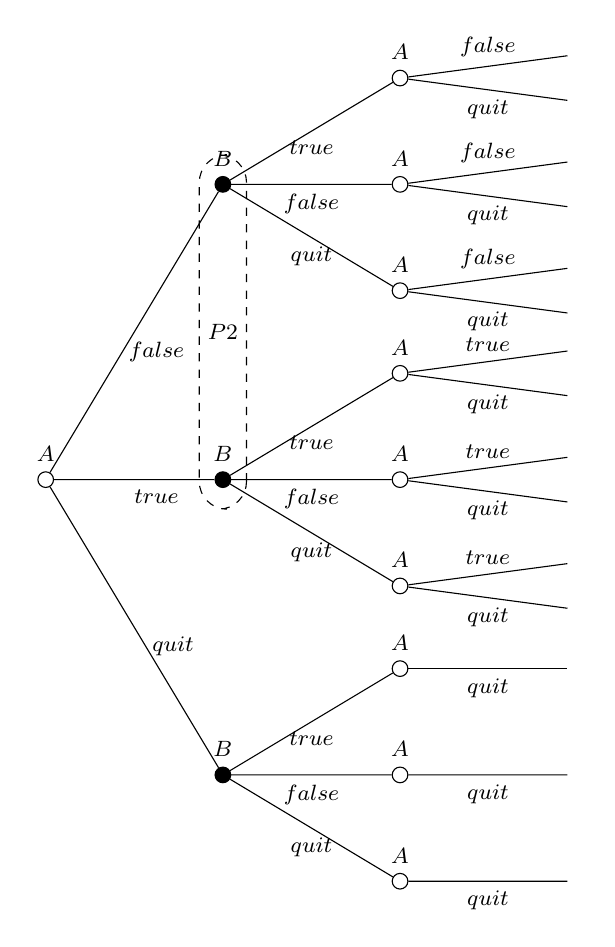
\begin{tikzpicture}[scale=1.5,font=\footnotesize, grow=right]
  % Specify spacing for each level of the tree
  \tikzstyle{level 1}=[level distance=15mm,sibling distance=25mm]
  \tikzstyle{level 2}=[level distance=15mm,sibling distance=9mm]
  \tikzstyle{level 3}=[level distance=15mm,sibling distance=4mm]
  % The Tree
  \node(0)[hollow node,label=above:{$A$}]{}
  child{node(1)[solid node,label=above:{$B$}]{}
    child{node[hollow node,label=above:{$A$}]{}
      child{node{} edge from parent node[below]{$quit$}}
      edge from parent node[below]{$quit$}
    }
    child{node[hollow node,label=above:{$A$}]{}
      child{node{} edge from parent node[below]{$quit$}}
      edge from parent node[below]{$false$}
    }
    child{node[hollow node,label=above:{$A$}]{}
      child{node{} edge from parent node[below]{$quit$}}
      edge from parent node[below]{$true$}
    }
    edge from parent node[below,xshift=14]{$quit$}
  }
  child{node(2)[solid node,label=above:{$B$}]{}
    child{node[hollow node,label=above:{$A$}]{}
      child{node{} edge from parent node[below]{$quit$}}
      child{node{} edge from parent node[above]{$true$}}
      edge from parent node[below]{$quit$}
    }
    child{node[hollow node,label=above:{$A$}]{}
      child{node{} edge from parent node[below]{$quit$}}
      child{node{} edge from parent node[above]{$true$}}
      edge from parent node[below]{$false$}
    }
    child{node[hollow node,label=above:{$A$}]{}
      child{node{} edge from parent node[below]{$quit$}}
      child{node{} edge from parent node[above]{$true$}}
      edge from parent node[below]{$true$}
    }
    edge from parent node[below,xshift=8]{$true$}
  }
  child{node(3)[solid node,label=above:{$B$}]{}
    child{node[hollow node,label=above:{$A$}]{}
      child{node{} edge from parent node[below]{$quit$}}
      child{node{} edge from parent node[above]{$false$}}
      edge from parent node[below]{$quit$}
    }
    child{node[hollow node,label=above:{$A$}]{}
      child{node{} edge from parent node[below]{$quit$}}
      child{node{} edge from parent node[above]{$false$}}
      edge from parent node[below]{$false$}
    }
    child{node[hollow node,label=above:{$A$}]{}
      child{node{} edge from parent node[below]{$quit$}}
      child{node{} edge from parent node[above]{$false$}}
      edge from parent node[below]{$true$}
    }
    edge from parent node[below,xshift=8]{$false$}
  };
  % information set
  \draw[dashed,rounded corners=10]($(2) + (.2,-.25)$)rectangle($(3) +(-.2,.25)$);
  % specify mover at 2nd information set
  \node at ($(2)!.5!(3)$) {$P2$};
\end{tikzpicture}

Simple parallel example is an OddEvens game. If we assume that neither side is taking the timed-risk of checking whether the other player has played, we can translate the OddsEvens game 
\lstinputlisting{../bilang/examples/OddsEvens.bi}

To the following extensive form:

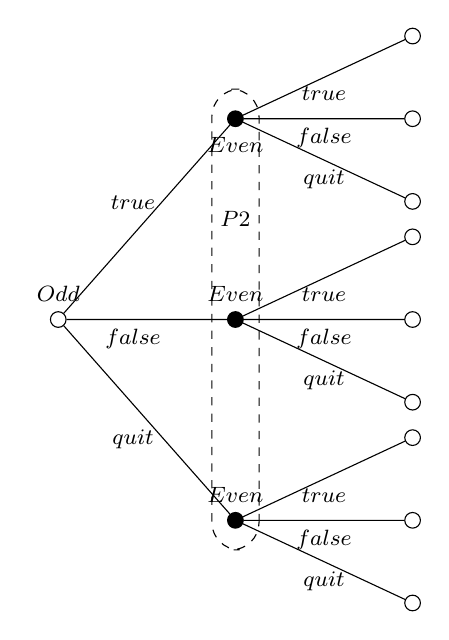
\begin{tikzpicture}[scale=1.5,font=\footnotesize, grow=right]
  % Specify spacing for each level of the tree
  \tikzstyle{level 1}=[level distance=15mm,sibling distance=17mm]
  \tikzstyle{level 2}=[level distance=15mm,sibling distance=7mm]
  % The Tree
  \node(0)[hollow node,label=above:{$Odd$}]{}
  child{node(1)[solid node,label=above:{$Even$}]{}
    child{node[hollow node]{} edge from parent node[below]{$quit$}}
    child{node[hollow node]{} edge from parent node[below]{$false$}}
    child{node[hollow node]{} edge from parent node[below]{$true$}}
    edge from parent node[below,xshift=-5]{$quit$}
  }
  child{node(2)[solid node,label=above:{$Even$}]{}
    child{node[hollow node]{} edge from parent node[below]{$quit$}}
    child{node[hollow node]{} edge from parent node[below]{$false$}}
    child{node[hollow node]{} edge from parent node[below]{$true$}}
    edge from parent node[below,xshift=-5]{$false$}
  }
  child{node(3)[solid node,label=below:{$Even$}]{}
    child{node[hollow node]{} edge from parent node[below]{$quit$}}
    child{node[hollow node]{} edge from parent node[below]{$false$}}
    child{node[hollow node]{} edge from parent node[below]{$true$}}
    edge from parent node[above,xshift=-5]{$true$}
  };
  % information set
  \draw[dashed,rounded corners=10]($(1) + (.2,-.25)$)rectangle($(3) +(-.2,.25)$);
  % specify mover at 2nd information set
  \node at ($(2)!.5!(3)$) {$P2$};
\end{tikzpicture}


Note that the games correspond only to certain types of extensive form games - ones that are implementable over blockchain. In particular, games are always perfect recall, by construction.

As another example we demonstrate Nash equilibria of the MontyHall game (with slightly different implementation), the OddsEvens game, and some others. This analysis reveals bugs and incentive problems, such as mishandling of quitting. Part of the resulting tree and analysis of the MontyHall game is shown below. Among other things, one can see that \texttt{undefined} values are not part of this specific equilibrium - which is a good sign.

\subsubsection{Multplayer Game}

\subsubsection{N-player Game}


\subsubsection{Absence of Communication Mismatches}
We use simple session types to do sanity check on the server code, and to verify the conformance of clients to the protocol. The program is translated to scribble code in a straightforward manner: \texttt{join}s are translated to \texttt{connect} actions between the server and the role, \texttt{yield} are translated to \texttt{send} with some arbitrary label, and then broadcast action to all the other roles, unless the \texttt{yield} was also \texttt{hidden}. In our language we allow no choice for the protocol, and no recursion, so these important options are left for future work; the scribble system is already equipped to handle these extensions.

The scribble protocol can then be used to verify the implementation of clients, in which case it is guaranteed (under our timing and fairness assumptions) that clients have no communication mismatches.

Scribble does not support unbounded number of roles yet, although the theory of session types has been extended to handle it. We can still produce a projection (local protocol) from a \textit{for yield} loop, since from the point of view of each client it is nothing but a simple send operation (clients are not intended to receive previous messages sent to the for loop). When the loop ends, the server broadcast the value of the variables updated inside the loop. So each local client will have a simple send-receive pair.

\subsection{Resource Analysis}
\subsubsection{Hidden Values}
A hidden variable can be seen as a resource: it is `allocated' when sent, `released' when revealed, and in the meantime cannot be copied. Unfortunately, a very useful pattern of resource usage -- a \texttt{using} or \texttt{with} construct -- is inappropriate since the variable is not used between the time it is committed to the time it is released, but only later; additionally, variables revealed in the meantime \textit{are} used later, so tying it to a scope is not useful at all. In a sense, the situation has more in common to an uninitialized variable, except that \textit{moving} the variables' value does make sense, and immediate initialization is not useful (it is just like a using public variable).

\subsubsection{Money}

\subsubsection{Connections}

Handling of connections (roles) is similar to standard resource handling in common imperative programming languages. Specifically, we tie connections to lexically scoped local variables, so when a role variable goes out of scope, the player tied to that role receives an appropriate notification.

\subsection{DQBF}
The language for full-information 2-player finite sequential games is QBF: for example the formula $\exists x \forall y: x > y$ refers to the game where the player chooses $x$ and shows it, then the opponent chooses $y$, and the first player wins iff $x > y$. Obviously the second player has a winning strategy, e.g. always choose $y=x$.

In QBF, there is a order of quantifiers define uniquely the information on which they depend; i.e. information dependency is a chain. In order to model partial information, we need to be able to specify a DAG of dependencies. DQBF consists of formulae of the form $\forall x_1, x_2, \ldots x_n \exists y_1 \{\overline{z_1}\}, y_2 \{\overline{z_2}\}, \ldots y_k \{\overline{z_k}\}: P(\overline{x}, \overline{y})$ where each $z_i$ is a list of variables on which $y_i$ depends. For example, the game $\exists x \forall y\{\}: x > y$ is the symmetric game in which both players make their choices independently; in this game the second player has no winning strategy.

In our case, it doesn't make sense to represent every dependency pattern, since many patterns do not make sense in our setting: we can only hide value (from everyone else) or reveal values (to everyone). In particular, the information flow graph must be transitive.

\section{Evaluation}

Finding a single Nash equilibrium in the MontyHall program takes roughly 80 minutes (after loading the game, which takes about 20 minutes).

\section{Related Work}

\section{Conclusion}

%% Acknowledgments
\begin{acks}                            %% acks environment is optional
                                        %% contents suppressed with 'anonymous'
  %% Commands \grantsponsor{<sponsorID>}{<name>}{<url>} and
  %% \grantnum[<url>]{<sponsorID>}{<number>} should be used to
  %% acknowledge financial support and will be used by metadata
  %% extraction tools.
  This material is based upon work supported by the
  \grantsponsor{GS100000001}{National Science
    Foundation}{http://dx.doi.org/10.13039/100000001} under Grant
  No.~\grantnum{GS100000001}{nnnnnnn} and Grant
  No.~\grantnum{GS100000001}{mmmmmmm}.  Any opinions, findings, and
  conclusions or recommendations expressed in this material are those
  of the author and do not necessarily reflect the views of the
  National Science Foundation.
\end{acks}


%% Bibliography
\bibliography{bibliography}


%% Appendix
\appendix
\section{Appendix}

Text of appendix \ldots

\end{document}
